\section{Canon and crosstalk}
\label{introduction:canon}

In cell biology, the big questions that we are interested in are generally imprecise.
For example, we may want to know: ``How does a
stem cell decide its fate?'' We cannot answer such questions directly, as they
are made up of an unknown number of sub-questions.
Such sub-questions that must first be addressed
include: What is a stem cell? What is a fate? And what does it
mean for a cell to ``decide''?

\subsubsection{Canon}

In practice, therefore, we typically begin with simpler and more
concrete questions, such as ``What factors influence cellular response $R$?''
where $R$ may be some property such as cell cycle arrest.
We can then screen for mutations, growth factors, or small molecules
that affect $R$, as measured using a convenient technology.
Here we are already limited in the experimental design by the variety
of the factors we have access to for testing against $R$. Further,
and perhaps more importantly, we are limited by what aspects of $R$
our technology can measure, and by not knowing whether we should even be
looking at $R$ at all.
But we must start somewhere, and so we begin to collect relationships
between experimental perturbations and measurements of $R$ for the
biological system we care about.


Over time, and across many laboratories,
we amass a library of knowledge consisting of
these experimental relationships. The meaning of each relationship alone, especially
at the beginning of the process, is fuzzy. In combination, however,
we hope that we can begin to build a model of how the biological system
works. Unfortunately, we do not know which of the perturbation-measurement
relationships are the most important, which are outright false, nor
which are only true under a particular set of experimental or biological
circumstances. We
work these disparate pieces of data into a general model
anyway, and allow that model to evolve along with our library of
knowledge, and take note of exceptions to the rules of the model. If enough
exceptions build up over time, models will sometimes emerge that can
better explain more of the data.


In the context of cellular signaling, this gradual process typically leads
to the development of so-called ``canonical'' signaling networks. These
networks are often constructed through the use of genetic experiments and
epistasis analysis, and then built upon by biochemical and other means.
Resulting canonical networks are typically depicted as protein \b{nodes} connected by
\b{edges} that carry some functional meaning, where that meaning might
be anything from the generic
``up-regulates'' to something more specific, for example an edge may mean
``phosphorylates residue $Y$, leading to ubiquitination and subsequent
degradation.''


Historical happenstance and available methodologies therefore play a large role in
how we define
canonical pathways. In cell and molecular biology education, we are often
taught cellular signaling through these canonical pathways
via the key experiments that laid their
foundations. We are therefore trained from the beginning to see the pathways as
non-overlapping, distinct channels of information
within cells that each carry out prototypical functions.


\subsubsection{Crosstalk}

However, once a canonical framework is in place, and is
generally accepted throughout the field, new findings must still
be attached to that framework. In this way, canonical networks tend to
continuously expand, eventually encroaching onto territory that once
belonged to some other canonical pathway
(see \ar{fig:introduction:complexity})  \cite{Kholodenko2006}.


  \begin{figure}[!bt]
  \centering
  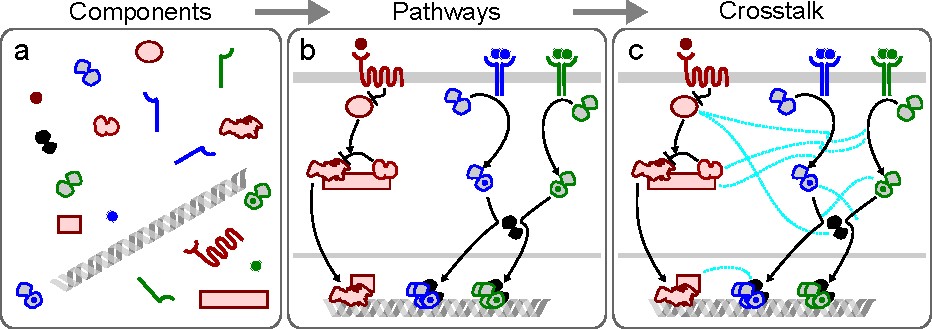
\includegraphics[width=6in]{FIGS/introduction/complexity.pdf}
  {\singlespacing 
  \caption[ Apparent signaling complexity increases over time.]
            { Apparent signaling complexity increases over time.
			\b{a}, Components of signaling pathways are typically discovered by
			genetic means or by treating cells with unknown, purified factors and
            observing the resulting phenotypes.
			\b{b}, These components are then organized into canonical signaling
			pathways based on epistasis experiments. \b{c}, Finally, canonical pathways
			are interconnected by new experiments whose results
			do not fit into the canonical framework. The network edges, as drawn here,
            may each have a different meaning and may be specific in time or to
            certain experimental contexts.}
  \label{fig:introduction:complexity}}
  \end{figure}


As canonical pathways send more and more tendrils into the global network,
we end up with models of cellular signaling wherein any perturbation
to the system ends up reverberating throughout the entire web: everything is
connected to everything. I refer to this phenomenon generally as ``crosstalk.''
While one may wonder how we can begin to address
such complexity, it is possible that the situation is less complex than we think.


An important aspect of these networks that is all too frequently ignored 
is \textbf{time}. The models that are sketched out
in any good review are static approximations of the true signaling
network. In effect, these static
networks are the maximum projections of a set of networks that exist across time
and across different experimental conditions. The actual network, evolving dynamically within
a cell as it processes information, might not ever look like the static map \arp{fig:introduction:xtalk}.


It is a rare experiment indeed that
measures all of the network edges simultaneously, as the goal
of most experiments is to flesh out a single edge or node. Therefore
we do not generally know if a given edge or node exists at all times, in all
systems, or if it is instead an ephemeral thing that comes and goes
as needed. Indeed, experimental evidence has demonstrated that the topologies of
signaling networks may not be constant, and that they may be
relatively simple at any instance in time \cite{Ideker2012,Ku2012}.


Aside from the missing temporal aspect in our static canonical networks
and inter-networks, there is another important and oft-ignored aspect.
That is, an edge is only useful for signaling if it
somehow transfers \b{information}. The purpose of a biochemical
signaling pathway is to carry information from one node to another.
The fact that two nodes are connected by a link, one that perhaps indicates binding
or phosphorylation, does not imply that information has been transferred.
Some edges between nodes may be tangential to the signaling process being studied,
or may be sending information into parallel signaling channels.
This information content problem should become clear later in this chapter and
in the particular case of signaling crosstalk reviewed in \autoref{pathways:introduction}
and studied in \ar{insulation:introduction}.


Instead of continually adding inter-network
edges, perhaps then we should carefully evaluate the edges
that already exist. By testing those edges across systems, at different times,
and explicitly verifying that they carry information, we may find that
some of these edges carry little weight and that therefore our
currently-complex view of signaling
must be both simplified and made dynamic in order to reflect reality.


  \begin{figure}[!bt]
  \centering
  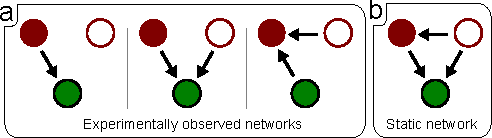
\includegraphics[width=4in]{FIGS/introduction/xtalk.pdf}
  {\singlespacing 
  \caption[Static networks may not represent true network behaviors.]
            { Static networks may not represent true network behaviors.
            \b{a}, Networks collected from multiple experimental conditions
            may show a variety of topologies. \b{b}, The static network
            diagrams that we typically draw are maximum projects or averages
            across the various experimentally observed topologies.}
  \label{fig:introduction:xtalk}}
  \end{figure}